% intro goes here. 

We present a $kD$ tree-based parallel strategy for solving with a {\it spacetime}-adaptive approach a general class of partial differential equations. This approach is primarily motivated by the necessity of designing computational methodologies that leverage the availability of very large computing clusters (exascale and beyond). For evolution problems, the standard approach of decomposing the spatial domain is a powerful paradigm of parallelization. However, for a fixed spatial discretization, the efficiency of purely spatial domain decomposition degrades substantially beyond a threshold -- usually tens of thousands of processors -- which makes this approach unsuitable on next generation machines. To overcome this barrier, a natural approach is to consider the time domain as an additional dimension and simultaneously solve for blocks of time, instead of the standard approach of sequential time-stepping. 

% \begin{figure*}[t]
%   \centering
%   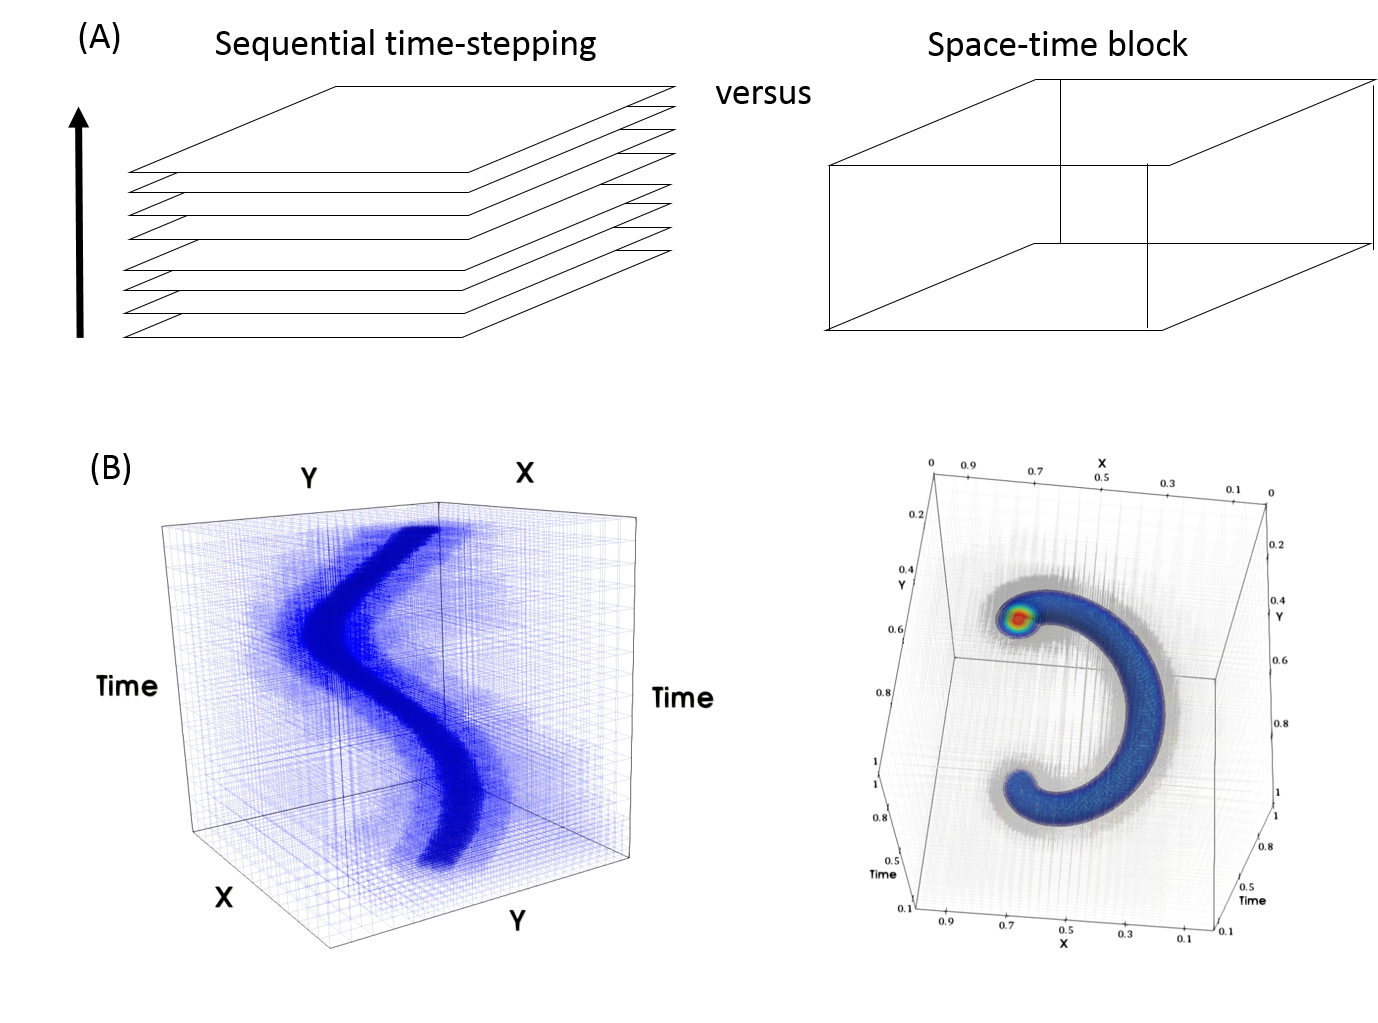
\includegraphics[width=0.7\textwidth]{figs/Picture2.png} \vspace{-0.35in}
%   \caption{\label{fig:Overview} {\small (A) Paradigm changing proposed work: Conventional approaches to computationally solving evolution equations rely on marching sequentially in time. This limits parallel scalability to the spatial domain. In contrast, we propose a paradigm breaking strategy of simultaneously solving for large blocks of spacetime. This will not only leverage next generation architectures, but will allow localized refinement in spacetime which will greatly streamline solution of a wide variety of evolution equations involving fronts and shocks. This opens up rich computational approaches for leveraging SPX: {\it a posteriori} error estimates, adjoints, preconditioner and solver designs as well as basic data structure design for solving problems in 4D space. (B) Preliminary results in $2D~\texttt{space} + 1D ~\texttt{time}$ dimensions (i.e. 3D spacetime) for a rotating heat source problem. Notice that the mesh is refined in {\bf spacetime} only in regions of interest. This not only guarantees accurate solutions in space {\bf and} time, but is also substantially more efficient than the strategy of taking very small time steps  necessary to guarantee temporal accuracy in the sequential approach.}} \vspace{-0.1in}
% \end{figure*}

This approach of solving for large blocks of spacetime is one of several promising approaches to time-parallel integration approaches that have been developed over the past century, but which are gaining increasing attention due to the availability of appropriate computing resources~\cite{50Years}. Broadly one can consider three types of parallelization approaches to solving a space-time problem. The first type of methods explicitly parallelizes only over time, and leaves spatial parallelism (and spatial adaptivity) undefined~\cite{parareal2001,falgout2014parallel}. These methods may also be considered as shooting methods~\cite{50Years}. The second type of methods explicitly parallelizes over space, and leaves temporal parallelism (and temporal adaptivity) undefined. These methods include wave form relaxation methods that attempt to reconcile the solution at spatial boundaries between space-time blocks~\cite{50Years}. The third type of methods explicitly targets parallelism (and adaptivity) in space and time. The current work seeks to advance type three methods. In the more narrow context of finite element methods, early work on type three methods was considered by Hughes and coworkers~\cite{hughes1996space,hughes1988space}, Tezduyar et al.~\cite{tezduyar2006space}, and Potanza and Reddy~\cite{pontaza2003spectral}, while variations on this theme have recently been explored by several groups~\cite{behr2008simplex, carey2010blockwise, lowrie1998space, mani2011efficient, rendall2012conservative, wang2015high}. 

%This approach of solving for large blocks of spacetime is one of several promising approaches to time parallel integration approaches that have been developed over the past century, but which are gaining increasing attention due to the availability of appropriate computing resources~\cite{50Years}. These include (a) shooting type time parallel methods that recursively improve 'initial' conditions at each time block ~\cite{parareal2001}, (b) wave form relaxation methods that attempt to reconcile solution at spatial boundaries between space time blocks, and (c) direct solutions in spacetime, where the complete spacetime block is discretized and reformulated into boundary value problems. 

Our preliminary work~\cite{dyja2018parallel} using the Finite Element Method (FEM) indicates that the third approach is particularly promising (see Fig.~\ref{fig:Overview}) as it provides a natural way to integrate mathematical analysis including construction of finite element error estimates (both {\it a priori} as well as {\it a posteriori}), and numerical stabilization of FEM solutions to advection-dominated equations, with foundation developments in scalable, parallel algorithms. The finite element method (FEM) is a widely popular numerical approach to solving partial differential equations, with multiple billions/year spent in CAD and CAM (computer aided design and manufacturing) based FEM software alone~\cite{Hughes_iso_book}. Its popularity arises from a compelling set of properties including (a) the ability to model arbitrary geometries, (b) the ability to seamlessly change order of representation (linear, quadratic and higher order), (c) the ability to utilize variational arguments that guarantee monotonic convergence to the solution with improved discretization, and (d) the ability to seamlessly utilize {\it a posteriori} error estimates to adapt the mesh. 

Solving for blocks of space-time provides a natural approach for effective usage of exascale computing resources~\cite{siam2013}, as well as leveraging novel architectures that exhibit extreme parallelism and deep memory hierarchies. In addition to this obvious advantage, this strategy provides the following advantages:
\begin{itemize}%[label={},nosep,leftmargin=1em,labelwidth=*,align=left]%\vspace{-0.15in}
    %\setlength\itemsep{0em}
    \item Solving for spacetime blocks also allows natural incorporation of {\it a posteriori} error estimates for spacetime mesh adaptivity. This has several additional tangible benefits in the context of computational overhead. For evolution problems -- including wave equations, and problems involving moving interfaces like bubbles and shocks -- that exhibit \text{``localized''} behavior in space and time, solving in blocks of spacetime that are locally refined to match the local behavior provides substantial computational gain~\cite{carey_estep}. An illustration (in lower dimensions) of this advantage (in $2D~\texttt{space} + 1D ~\texttt{time}$) is shown in Fig.~\ref{fig:Overview}(B), where the refined mesh is localized along the regions of high gradient of the solution.
    \item Solving in spacetime provides easy access to the full time history of the solution which is essential for the solution of design/inverse problems involving adjoints~\cite{Baskar1,Baskar2}
    \item Solving PDE's in spacetime removes any time-stepping constraints (like the CFL condition) on the numerical approach as the solution across all time-steps are simultaneously solved. This concept is illustrated in Fig.~\ref{fig:Overview}(B). The temporal discretization far away from the oscillating source is $2^5$ times larger than the smallest temporal discretization. This large variation in time step has no impact on numerical stability, which is an advantage over conventional sequential time stepping approaches.
    \item Finally, considering time as an additional dimension allows us to harness the benefits of using higher order basis functions to get high order accurate temporal schemes for no additional implementation cost (since these basis functions are already available for the spatial discretization). We derive theoretical {\it a priori} estimates of convergence with basis order and mesh size, and show that temporal error scales as a power of the mesh size in space time $|u - u_e|_2 \leq Ch^{\alpha}$, where $\alpha = \texttt{order of basis function} + 1$. Fig.~\ref{fig:ST_conv} computationally illustrates this point. We solve a 2D transient problem in spacetime on a 3D mesh. Using cubic basis functions is equivalent to a multi-step fourth order Runge-Kutta scheme for the sequential time stepping problem. 
\end{itemize}

\begin{figure}%{r}{0.5\textwidth}
\vspace{-0.2in}
  \begin{center}
 % \hspace{-3in}
    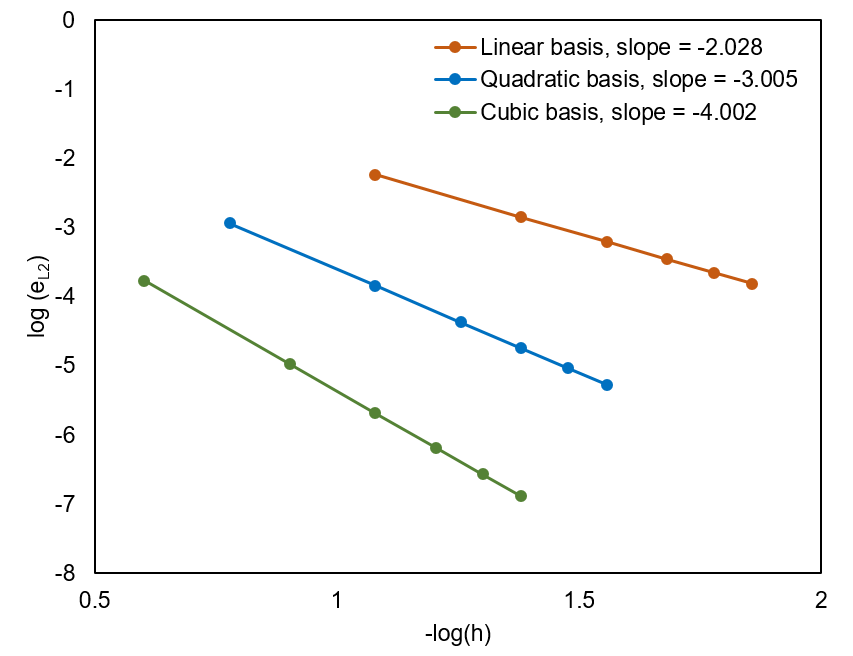
\includegraphics[trim={0 0 0 0},clip,width=0.48\textwidth]{figs/cnv-NL-final-time}
  \end{center}
   \vspace{-0.1in}
   \caption{\label{fig:ST_conv} \small Considering time to be another dimension allows easy use of higher order basis functions to get high order temporal accuracy. The figure illustrates how switching from linear to quadratic to cubic basis functions (for the problem solved in  Fig.~\ref{fig:Overview}B) in spacetime is equivalent to multi-step Runge Kutta methods of order 2, 3 and 4, respectively. }
   \vspace{-0.1in}
\end{figure}

\par Additionally, we break mesh-based abstractions for performing finite element (FEM) computations on adaptive spacetime meshes with the objective of achieving high performance and scalability on current and future architectures with extreme levels of parallelism and deep memory hierarchies. The new abstractions are designed to support matrix-free abstractions since these are important for large-scale parallelism. In addition, the new abstractions will enable code portability, for both CPU and GPU architectures. 

Our contributions in this paper are as follows: 
(a) we develop efficient $4D$ adaptive mesh construction and 2:1 balancing algorithms, 
(b) we develop a mesh-free matrix-free algorithms for finite element computations using a spacetime formulation, 
(c)  we derive both {\it a priori} error estimates, as well as residual based {\it a posteriori} error estimates for a canonical problem -- the linear time dependent heat diffusion equation, and numerically illustrate the theoretically determined improved convergence behavior of the space-time solution approach, and 
(d) we compare the scaling behavior of sequential time stepping method with the space-time approach. %the Crank Nicholson time - stepping method with the coupled space - time formulation for the linear diffusion equation with linear basis function.  

%Additionally, we formulate the \textit{aposteriori} error estimate for the coupled space - time formulation for the diffusion equations.  


%Our goal is to evaluate using x64, Intel Xeon Phi, Power8/9 and nVidia GPUs. In addition, since several linear solvers - such as geometric multigrid - depend on mesh information, we will develop solver realizations for our mesh-free abstractions.

%Finally, the outcome of this abstraction breaking approach to rethink FEM simulations of partial differential equations will be illustrated using two very impactful application examples in (a) flow and charge transport in complex heterogeneous porous films (energy harvesting)~\cite{kodali2012computer,kodali2012computational,wodo2015automated}, and (b) rapid evaluation of contaminant dispersal in urban neighborhoods~\cite{fontanini2017contaminant,fontanini2016methodology} (infrastructure and safety). This integration of a paradigm shifting approach to scientific computing with targeted, societally impactful applications is driven by the NSF mandate on Convergence thinking.
